\section{The uncertain Darcy problem}
The methods for approximating the mean exit time have been investigated in a general frame. In the following we will consider \eqref{eq:GeneralModel} with $f\colon \mathbb{R}^2 \rightarrow \mathbb{R}^2$ given by the solution of the uncertain Darcy problem. 

\subsection{Problem statement}
Let us consider a domain $D \subset \mathbb{R}^2$. Let us define the Neumann boundaries of $D$ as $\Gamma_N$, its inlet boundary as $\Gamma_{in}$ and its outlet boundary as $\Gamma_{out}$. Then, we search the solution of the following problem
\begin{equation}
	\label{eq:DarcyProblem}
	\left \{
  	\begin{aligned}
		u &= -A \nabla p, && \text{in } D, \\
		\nabla\cdot u &= 0, && \text{in } D, \\
		p &= p_0, && \text{on } \Gamma_{in},\\
		p &= 0, && \text{on } \Gamma_{out}, \\
		\nabla p &= 0, && \text{on } \Gamma_N,
	\end{aligned} \right.
\end{equation}
where $A$ is a random field. The solution $u$ of this equation is used as transport field in equation \eqref{eq:GeneralModel}, which can be therefore written as
\begin{equation}\label{eq:GeneralDarcySDE}
  	\left \{
  	\begin{aligned}
    		dX(t) &= u(X) dt + \sigma dW(t), && 0 < t \leq T, \\
    		X(0)  &= X_0, 	 	     && X_0 \in D,
  	\end{aligned} \right.
\end{equation} 
where we set the boundary conditions to be reflecting on $\Gamma_N$ and killing on both $\Gamma_{in},\Gamma_{out}$.

\begin{figure}[t]
    \centering
    \begin{subfigure}{0.49\linewidth}
        \centering
        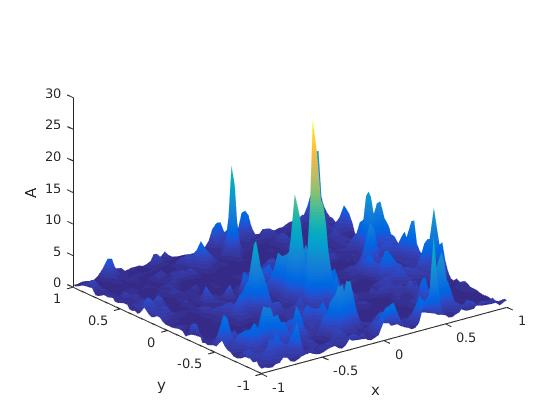
\includegraphics [width=1\linewidth]{Darcy/Pictures/A.jpg}
        \caption{Random field.}
        \label{fig:DarcyA}
    \end{subfigure}
    \begin{subfigure}{0.49\linewidth}
        \centering
        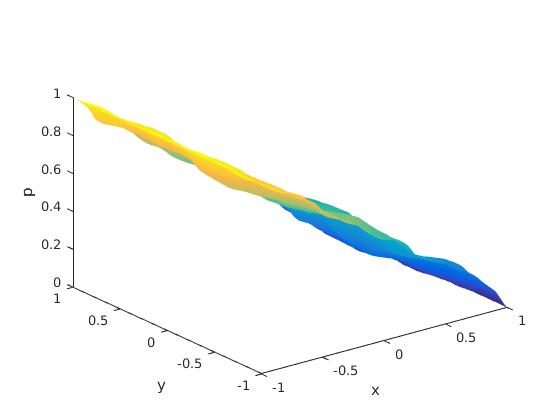
\includegraphics [width=1\linewidth]{Darcy/Pictures/P.jpg}
        \caption{Pressure field.}
        \label{fig:DarcyP}
    \end{subfigure}    
    \begin{subfigure}{0.49\linewidth}
        \centering
        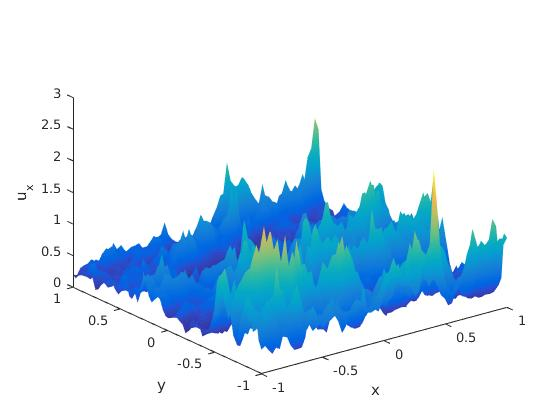
\includegraphics [width=1\linewidth]{Darcy/Pictures/Ux.jpg}
        \caption{$x$ component of velocity field.}
        \label{fig:DarcyUx}
    \end{subfigure}
    \begin{subfigure}{0.49\linewidth}
        \centering
        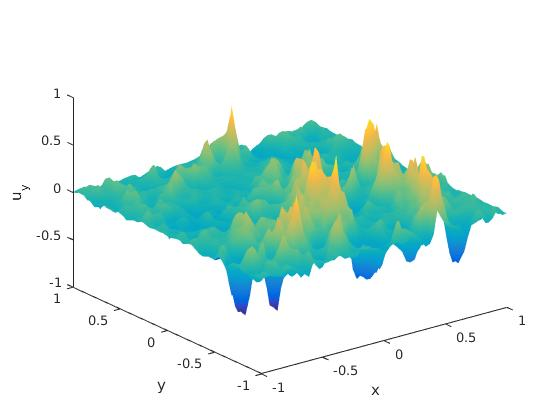
\includegraphics [width=1\linewidth]{Darcy/Pictures/Uy.jpg}
        \caption{$y$ component of velocity field.}
        \label{fig:DarcyUy}
    \end{subfigure}    
    \caption{Approximate solution of the uncertain Darcy problem.}
    \label{fig:DarcyResults}
\end{figure}



\subsection{Finite Elements solution of the Darcy problem}

Let us consider the domain $D = [-1,1]^2$. The random field $A$ in \eqref{eq:DarcyProblem} is chosen to be lognormal, \textit{i.e.}, 
\begin{equation}\label{eq:RandomField}
	A = e^\gamma,
\end{equation}
where $\gamma$ is a normal random field defined by its covariance function $\mathrm{cov}_\gamma(x_1,x_2)$ for any couple of points $x_1,x_2$ in the domain $D$. The covariance function is of the Matern family \cite{Nobile2015}, thus having the following form
\begin{equation}\label{eq:CovFunction}
	\mathrm{cov}_\gamma(x_1,x_2) = \frac{\sigma_A^2}{\Gamma(\nu)2^{\nu-1}}\Big(\sqrt{2\nu}\frac{|x_1-x_2|}{L_c}\Big)^\nu K_{\nu}\Big(\sqrt{2\nu}\frac{|x_1-x_2|}{L_c}\Big), \quad \nu \geq 0.5,
\end{equation}
where $\sigma_A^2$ is the variance, $L_c$ is the correlation length, $\Gamma$ is the gamma function, $K_\nu$ is the modified Bessel function of the second kind and $\nu$ is a parameter. Let us remark that the covariance function does not depend on $x_1, x_2$ but only on their euclidean distance $|x_1 - x_2|$. The regularity of the covariance function and of the realizations of $A$ depend on $\nu$. In particular each realization of the field $A$ is $\alpha$-Hölder continuous for $0 < \alpha < \nu$. Therefore, for $\nu = 1 + \epl, \epl > 0$, the random field is Lipschitz continuous. Results concerning further regularity properties of $A$ can be found in \cite{Nobile2015}. The realizations of $A$ are computed using a discrete Fourier transformation on the vertices of a grid of $D$, equispaced on both the $x$ and $y$ directions with the same spacing $\Delta_A$. Then, the numerical solution $\hat{p}$ of \eqref{eq:DarcyProblem} is obtained with linear Finite Elements on a regular mesh $T_p$ with maximum element size $\Delta_p$. Since the vertices of the grid on which we compute $A$ do not coincide with the vertices of $T_p$, we interpolate $A$ on $T_p$. Then, the velocity field $\hat{u}$ is retrived computing the gradient of $\hat{p}$ as in equation \eqref{eq:DarcyProblem}. We choose to perform this procedure using the scientific software \texttt{FreeFem++}. The results for a realization of $A$ are shown in Figure \ref{fig:DarcyResults}, where the value of the inlet pressure $p_0$ is equal to 1, and the parameters for the random field are $\nu = 0.5, L_c = 0.05$. 


\subsection{Solution of the SDE}

Once the Finite Element approximation $\hat{u}$ of the velocity field is available, it is possible to approximate by means of DEM and CEM the solution of \eqref{eq:GeneralDarcySDE}. The values of the numerical solution $X_h$ can take any value in $D$, therefore it is necessary that the velocity field is defined in any point in $D$. If an interpolation of $\hat{u}$ is performed at each step, both DEM and CEM lose in computational efficiency. Hence, an interpolation of $\hat{u}$ has to be performed before the numerical integration of the SDE. Therefore, we define a grid with spacing $\Delta_u$, interpolating the values of $\hat{u}$ in the center of each square defined by the grid (Figure \ref{fig:GridVelocity}). Let us denote by $Q$ the set of the interpolation points, whose elements are defined by
\begin{equation}\label{eq:InterpMatrix}
	\{Q\}_{ij} = \begin{pmatrix} -1 + (i-0.5)\Delta_u, & -1 + (j-0.5)\Delta_u \end{pmatrix}^T, \quad i,j = 1, \dots, \frac{2}{\Delta_u} =: N_u.
\end{equation}
We compute two matrices $U_x, U_y$ of $\mathbb{R}^{N_u \times N_u}$ containing the values of the two components of $\hat{u}$ interpolated on the points of $Q$. Then, the velocity field is considered to be piecewise constant in each square of the grid defined by $\Delta_u$. Therefore, if we denote by $\tilde{u}$ the transport field for the SDE, at the $i$-th step of the integration $\tilde{u}$ is evaluated as follows
\begin{equation}\label{eq:VelEval}
	\tilde{u}(X_h(t_i)) = \begin{pmatrix}	U_x(\ceil{(X_{h,1}(t_i)+1)/\Delta_u},\ceil{(X_{h,2}(t_i)+1)/\Delta_u}) \\
					U_y(\ceil{(X_{h,1}(t_i)+1)/\Delta_u},\ceil{(X_{h,2}(t_i)+1)/\Delta_u}) \end{pmatrix},
\end{equation}
where $X_{h,1}, X_{h,2}$ denote the first and second components of $X_h$ and $U_x(i,j)$ represents the element $(i,j)$ of the matrix $U_x$ (respectively $U_y$). Let us remark that this operation involves only an evaluation of a matrix at each timestep, which is an operation of negligible computational cost. This implies a relevant improvement with respect to interpolating the solution at each timestep, which is on the other side a costly operation. Then, given the step size $h$, one step of DEM will be defined as
\begin{equation}\label{eq:DEMDarcy}
	X^d_{h,i+1} = \tilde{u}(X^d_{h,i}) h + \sigma (W(t_{i+1}) - W(t_i)).
\end{equation}
Given an input initial value $X_0$ for \eqref{eq:GeneralDarcySDE}, we approximate the solution using DEM and CEM using the strategy above. The theoretical investigation presented in Section 3 guarantees that if the interpolation and the element size chosen for the Finite Element approximation tend to zero, the solution will tend to the exact solution of \eqref{eq:DarcyProblem} for each realization of $A$. Unfortunately, the requirements of smoothness that we included in Section 3 are not satisfied by the solution of \eqref{eq:DarcyProblem}, unless $\nu$ is strictly bigger than one, as the random field and therefore the solution $u$ would be Lipschitz continuous. We hope that numerically the solution will in practice provide reasonable results even for a rough transport field. In Figure \ref{fig:TrajSDEDarcy} we display fifteen trajectories for $X_0 = (-0.8,-0.8)^T$ with two different step sizes. The choice of the initial point is made in order to observe reflections on the lower boundary of the domain $D$ on which we compute the solution, as well as the killing boundary at the right side. 

\begin{figure}[t]
    \centering
    \resizebox{0.6\linewidth}{!}{% This file was created by matlab2tikz.
%
%The latest updates can be retrieved from
%  http://www.mathworks.com/matlabcentral/fileexchange/22022-matlab2tikz-matlab2tikz
%where you can also make suggestions and rate matlab2tikz.
%
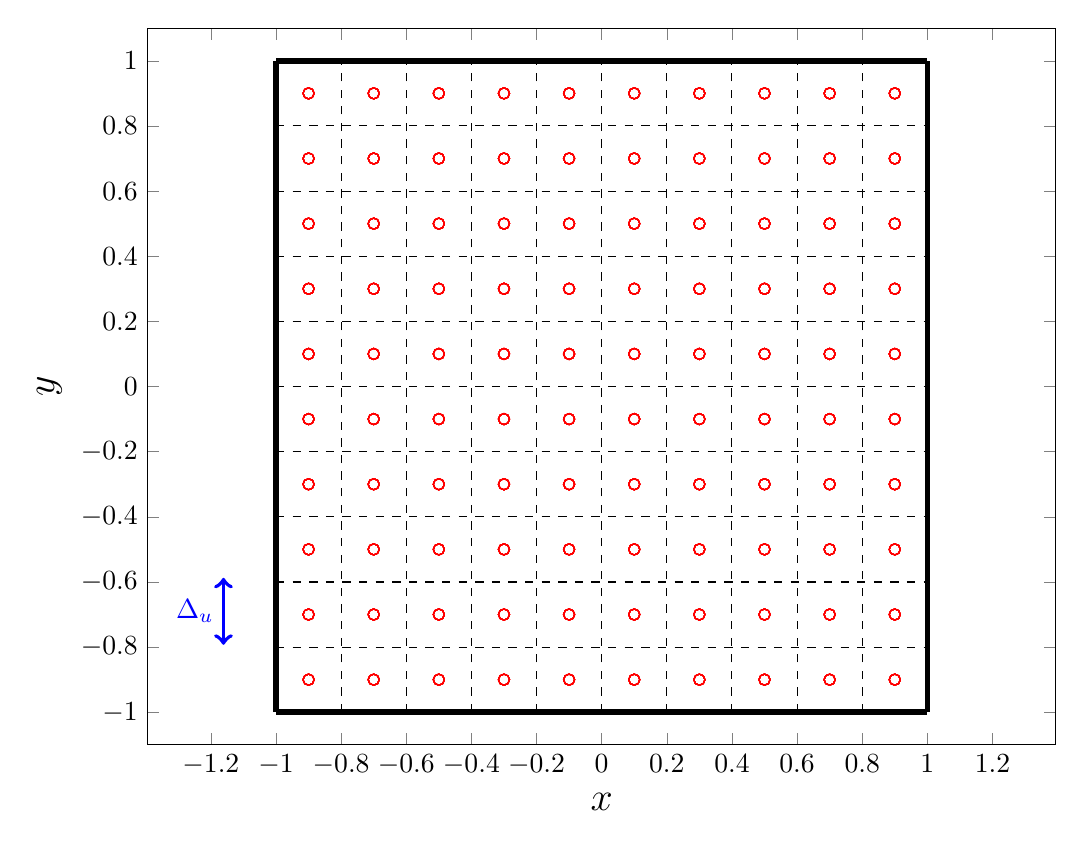
\begin{tikzpicture}



\begin{axis}[%
width=4.542in,
height=3.583in,
at={(0.801in,0.484in)},
scale only axis,
xmin=-1.39468302658487,
xmax=1.39468302658487,
xlabel={$x$},
xlabel style={font=\Large},
ymin=-1.1,
ymax=1.1,
ylabel={$y$},
ylabel style={font=\Large},
axis background/.style={fill=white}
]
\addplot [color=black,solid,line width=2.0pt,forget plot]
  table[row sep=crcr]{%
-1	-1\\
-1	1\\
};
\addplot [color=black,solid,line width=2.0pt,forget plot]
  table[row sep=crcr]{%
1	-1\\
1	1\\
};
\addplot [color=black,solid,line width=2.0pt,forget plot]
  table[row sep=crcr]{%
-1	-1\\
1	-1\\
};
\addplot [color=black,solid,line width=2.0pt,forget plot]
  table[row sep=crcr]{%
-1	1\\
1	1\\
};
\addplot [color=black,dashed,forget plot]
  table[row sep=crcr]{%
-1	-0.8\\
1	-0.8\\
};
\addplot [color=black,dashed,forget plot]
  table[row sep=crcr]{%
-0.8	-1\\
-0.8	1\\
};
\addplot [color=red,only marks,mark=o,mark options={solid},forget plot]
  table[row sep=crcr]{%
-0.9	-0.9\\
-0.9	-0.7\\
-0.9	-0.5\\
-0.9	-0.3\\
-0.9	-0.1\\
-0.9	0.1\\
-0.9	0.3\\
-0.9	0.5\\
-0.9	0.7\\
-0.9	0.9\\
};
\addplot [color=red,only marks,mark=o,mark options={solid},forget plot]
  table[row sep=crcr]{%
-0.9	-0.9\\
-0.9	-0.7\\
-0.9	-0.5\\
-0.9	-0.3\\
-0.9	-0.1\\
-0.9	0.1\\
-0.9	0.3\\
-0.9	0.5\\
-0.9	0.7\\
-0.9	0.9\\
};
\addplot [color=red,only marks,mark=o,mark options={solid},forget plot]
  table[row sep=crcr]{%
-0.9	-0.9\\
-0.9	-0.7\\
-0.9	-0.5\\
-0.9	-0.3\\
-0.9	-0.1\\
-0.9	0.1\\
-0.9	0.3\\
-0.9	0.5\\
-0.9	0.7\\
-0.9	0.9\\
};
\addplot [color=red,only marks,mark=o,mark options={solid},forget plot]
  table[row sep=crcr]{%
-0.9	-0.9\\
-0.9	-0.7\\
-0.9	-0.5\\
-0.9	-0.3\\
-0.9	-0.1\\
-0.9	0.1\\
-0.9	0.3\\
-0.9	0.5\\
-0.9	0.7\\
-0.9	0.9\\
};
\addplot [color=red,only marks,mark=o,mark options={solid},forget plot]
  table[row sep=crcr]{%
-0.9	-0.9\\
-0.9	-0.7\\
-0.9	-0.5\\
-0.9	-0.3\\
-0.9	-0.1\\
-0.9	0.1\\
-0.9	0.3\\
-0.9	0.5\\
-0.9	0.7\\
-0.9	0.9\\
};
\addplot [color=red,only marks,mark=o,mark options={solid},forget plot]
  table[row sep=crcr]{%
-0.9	-0.9\\
-0.9	-0.7\\
-0.9	-0.5\\
-0.9	-0.3\\
-0.9	-0.1\\
-0.9	0.1\\
-0.9	0.3\\
-0.9	0.5\\
-0.9	0.7\\
-0.9	0.9\\
};
\addplot [color=red,only marks,mark=o,mark options={solid},forget plot]
  table[row sep=crcr]{%
-0.9	-0.9\\
-0.9	-0.7\\
-0.9	-0.5\\
-0.9	-0.3\\
-0.9	-0.1\\
-0.9	0.1\\
-0.9	0.3\\
-0.9	0.5\\
-0.9	0.7\\
-0.9	0.9\\
};
\addplot [color=red,only marks,mark=o,mark options={solid},forget plot]
  table[row sep=crcr]{%
-0.9	-0.9\\
-0.9	-0.7\\
-0.9	-0.5\\
-0.9	-0.3\\
-0.9	-0.1\\
-0.9	0.1\\
-0.9	0.3\\
-0.9	0.5\\
-0.9	0.7\\
-0.9	0.9\\
};
\addplot [color=red,only marks,mark=o,mark options={solid},forget plot]
  table[row sep=crcr]{%
-0.9	-0.9\\
-0.9	-0.7\\
-0.9	-0.5\\
-0.9	-0.3\\
-0.9	-0.1\\
-0.9	0.1\\
-0.9	0.3\\
-0.9	0.5\\
-0.9	0.7\\
-0.9	0.9\\
};
\addplot [color=red,only marks,mark=o,mark options={solid},forget plot]
  table[row sep=crcr]{%
-0.9	-0.9\\
-0.9	-0.7\\
-0.9	-0.5\\
-0.9	-0.3\\
-0.9	-0.1\\
-0.9	0.1\\
-0.9	0.3\\
-0.9	0.5\\
-0.9	0.7\\
-0.9	0.9\\
};
\addplot [color=black,dashed,forget plot]
  table[row sep=crcr]{%
-1	-0.6\\
1	-0.6\\
};
\addplot [color=black,dashed,forget plot]
  table[row sep=crcr]{%
-0.6	-1\\
-0.6	1\\
};
\addplot [color=red,only marks,mark=o,mark options={solid},forget plot]
  table[row sep=crcr]{%
-0.7	-0.9\\
-0.7	-0.7\\
-0.7	-0.5\\
-0.7	-0.3\\
-0.7	-0.1\\
-0.7	0.1\\
-0.7	0.3\\
-0.7	0.5\\
-0.7	0.7\\
-0.7	0.9\\
};
\addplot [color=red,only marks,mark=o,mark options={solid},forget plot]
  table[row sep=crcr]{%
-0.7	-0.9\\
-0.7	-0.7\\
-0.7	-0.5\\
-0.7	-0.3\\
-0.7	-0.1\\
-0.7	0.1\\
-0.7	0.3\\
-0.7	0.5\\
-0.7	0.7\\
-0.7	0.9\\
};
\addplot [color=red,only marks,mark=o,mark options={solid},forget plot]
  table[row sep=crcr]{%
-0.7	-0.9\\
-0.7	-0.7\\
-0.7	-0.5\\
-0.7	-0.3\\
-0.7	-0.1\\
-0.7	0.1\\
-0.7	0.3\\
-0.7	0.5\\
-0.7	0.7\\
-0.7	0.9\\
};
\addplot [color=red,only marks,mark=o,mark options={solid},forget plot]
  table[row sep=crcr]{%
-0.7	-0.9\\
-0.7	-0.7\\
-0.7	-0.5\\
-0.7	-0.3\\
-0.7	-0.1\\
-0.7	0.1\\
-0.7	0.3\\
-0.7	0.5\\
-0.7	0.7\\
-0.7	0.9\\
};
\addplot [color=red,only marks,mark=o,mark options={solid},forget plot]
  table[row sep=crcr]{%
-0.7	-0.9\\
-0.7	-0.7\\
-0.7	-0.5\\
-0.7	-0.3\\
-0.7	-0.1\\
-0.7	0.1\\
-0.7	0.3\\
-0.7	0.5\\
-0.7	0.7\\
-0.7	0.9\\
};
\addplot [color=red,only marks,mark=o,mark options={solid},forget plot]
  table[row sep=crcr]{%
-0.7	-0.9\\
-0.7	-0.7\\
-0.7	-0.5\\
-0.7	-0.3\\
-0.7	-0.1\\
-0.7	0.1\\
-0.7	0.3\\
-0.7	0.5\\
-0.7	0.7\\
-0.7	0.9\\
};
\addplot [color=red,only marks,mark=o,mark options={solid},forget plot]
  table[row sep=crcr]{%
-0.7	-0.9\\
-0.7	-0.7\\
-0.7	-0.5\\
-0.7	-0.3\\
-0.7	-0.1\\
-0.7	0.1\\
-0.7	0.3\\
-0.7	0.5\\
-0.7	0.7\\
-0.7	0.9\\
};
\addplot [color=red,only marks,mark=o,mark options={solid},forget plot]
  table[row sep=crcr]{%
-0.7	-0.9\\
-0.7	-0.7\\
-0.7	-0.5\\
-0.7	-0.3\\
-0.7	-0.1\\
-0.7	0.1\\
-0.7	0.3\\
-0.7	0.5\\
-0.7	0.7\\
-0.7	0.9\\
};
\addplot [color=red,only marks,mark=o,mark options={solid},forget plot]
  table[row sep=crcr]{%
-0.7	-0.9\\
-0.7	-0.7\\
-0.7	-0.5\\
-0.7	-0.3\\
-0.7	-0.1\\
-0.7	0.1\\
-0.7	0.3\\
-0.7	0.5\\
-0.7	0.7\\
-0.7	0.9\\
};
\addplot [color=red,only marks,mark=o,mark options={solid},forget plot]
  table[row sep=crcr]{%
-0.7	-0.9\\
-0.7	-0.7\\
-0.7	-0.5\\
-0.7	-0.3\\
-0.7	-0.1\\
-0.7	0.1\\
-0.7	0.3\\
-0.7	0.5\\
-0.7	0.7\\
-0.7	0.9\\
};
\addplot [color=black,dashed,forget plot]
  table[row sep=crcr]{%
-1	-0.4\\
1	-0.4\\
};
\addplot [color=black,dashed,forget plot]
  table[row sep=crcr]{%
-0.4	-1\\
-0.4	1\\
};
\addplot [color=red,only marks,mark=o,mark options={solid},forget plot]
  table[row sep=crcr]{%
-0.5	-0.9\\
-0.5	-0.7\\
-0.5	-0.5\\
-0.5	-0.3\\
-0.5	-0.1\\
-0.5	0.1\\
-0.5	0.3\\
-0.5	0.5\\
-0.5	0.7\\
-0.5	0.9\\
};
\addplot [color=red,only marks,mark=o,mark options={solid},forget plot]
  table[row sep=crcr]{%
-0.5	-0.9\\
-0.5	-0.7\\
-0.5	-0.5\\
-0.5	-0.3\\
-0.5	-0.1\\
-0.5	0.1\\
-0.5	0.3\\
-0.5	0.5\\
-0.5	0.7\\
-0.5	0.9\\
};
\addplot [color=red,only marks,mark=o,mark options={solid},forget plot]
  table[row sep=crcr]{%
-0.5	-0.9\\
-0.5	-0.7\\
-0.5	-0.5\\
-0.5	-0.3\\
-0.5	-0.1\\
-0.5	0.1\\
-0.5	0.3\\
-0.5	0.5\\
-0.5	0.7\\
-0.5	0.9\\
};
\addplot [color=red,only marks,mark=o,mark options={solid},forget plot]
  table[row sep=crcr]{%
-0.5	-0.9\\
-0.5	-0.7\\
-0.5	-0.5\\
-0.5	-0.3\\
-0.5	-0.1\\
-0.5	0.1\\
-0.5	0.3\\
-0.5	0.5\\
-0.5	0.7\\
-0.5	0.9\\
};
\addplot [color=red,only marks,mark=o,mark options={solid},forget plot]
  table[row sep=crcr]{%
-0.5	-0.9\\
-0.5	-0.7\\
-0.5	-0.5\\
-0.5	-0.3\\
-0.5	-0.1\\
-0.5	0.1\\
-0.5	0.3\\
-0.5	0.5\\
-0.5	0.7\\
-0.5	0.9\\
};
\addplot [color=red,only marks,mark=o,mark options={solid},forget plot]
  table[row sep=crcr]{%
-0.5	-0.9\\
-0.5	-0.7\\
-0.5	-0.5\\
-0.5	-0.3\\
-0.5	-0.1\\
-0.5	0.1\\
-0.5	0.3\\
-0.5	0.5\\
-0.5	0.7\\
-0.5	0.9\\
};
\addplot [color=red,only marks,mark=o,mark options={solid},forget plot]
  table[row sep=crcr]{%
-0.5	-0.9\\
-0.5	-0.7\\
-0.5	-0.5\\
-0.5	-0.3\\
-0.5	-0.1\\
-0.5	0.1\\
-0.5	0.3\\
-0.5	0.5\\
-0.5	0.7\\
-0.5	0.9\\
};
\addplot [color=red,only marks,mark=o,mark options={solid},forget plot]
  table[row sep=crcr]{%
-0.5	-0.9\\
-0.5	-0.7\\
-0.5	-0.5\\
-0.5	-0.3\\
-0.5	-0.1\\
-0.5	0.1\\
-0.5	0.3\\
-0.5	0.5\\
-0.5	0.7\\
-0.5	0.9\\
};
\addplot [color=red,only marks,mark=o,mark options={solid},forget plot]
  table[row sep=crcr]{%
-0.5	-0.9\\
-0.5	-0.7\\
-0.5	-0.5\\
-0.5	-0.3\\
-0.5	-0.1\\
-0.5	0.1\\
-0.5	0.3\\
-0.5	0.5\\
-0.5	0.7\\
-0.5	0.9\\
};
\addplot [color=red,only marks,mark=o,mark options={solid},forget plot]
  table[row sep=crcr]{%
-0.5	-0.9\\
-0.5	-0.7\\
-0.5	-0.5\\
-0.5	-0.3\\
-0.5	-0.1\\
-0.5	0.1\\
-0.5	0.3\\
-0.5	0.5\\
-0.5	0.7\\
-0.5	0.9\\
};
\addplot [color=black,dashed,forget plot]
  table[row sep=crcr]{%
-1	-0.2\\
1	-0.2\\
};
\addplot [color=black,dashed,forget plot]
  table[row sep=crcr]{%
-0.2	-1\\
-0.2	1\\
};
\addplot [color=red,only marks,mark=o,mark options={solid},forget plot]
  table[row sep=crcr]{%
-0.3	-0.9\\
-0.3	-0.7\\
-0.3	-0.5\\
-0.3	-0.3\\
-0.3	-0.1\\
-0.3	0.1\\
-0.3	0.3\\
-0.3	0.5\\
-0.3	0.7\\
-0.3	0.9\\
};
\addplot [color=red,only marks,mark=o,mark options={solid},forget plot]
  table[row sep=crcr]{%
-0.3	-0.9\\
-0.3	-0.7\\
-0.3	-0.5\\
-0.3	-0.3\\
-0.3	-0.1\\
-0.3	0.1\\
-0.3	0.3\\
-0.3	0.5\\
-0.3	0.7\\
-0.3	0.9\\
};
\addplot [color=red,only marks,mark=o,mark options={solid},forget plot]
  table[row sep=crcr]{%
-0.3	-0.9\\
-0.3	-0.7\\
-0.3	-0.5\\
-0.3	-0.3\\
-0.3	-0.1\\
-0.3	0.1\\
-0.3	0.3\\
-0.3	0.5\\
-0.3	0.7\\
-0.3	0.9\\
};
\addplot [color=red,only marks,mark=o,mark options={solid},forget plot]
  table[row sep=crcr]{%
-0.3	-0.9\\
-0.3	-0.7\\
-0.3	-0.5\\
-0.3	-0.3\\
-0.3	-0.1\\
-0.3	0.1\\
-0.3	0.3\\
-0.3	0.5\\
-0.3	0.7\\
-0.3	0.9\\
};
\addplot [color=red,only marks,mark=o,mark options={solid},forget plot]
  table[row sep=crcr]{%
-0.3	-0.9\\
-0.3	-0.7\\
-0.3	-0.5\\
-0.3	-0.3\\
-0.3	-0.1\\
-0.3	0.1\\
-0.3	0.3\\
-0.3	0.5\\
-0.3	0.7\\
-0.3	0.9\\
};
\addplot [color=red,only marks,mark=o,mark options={solid},forget plot]
  table[row sep=crcr]{%
-0.3	-0.9\\
-0.3	-0.7\\
-0.3	-0.5\\
-0.3	-0.3\\
-0.3	-0.1\\
-0.3	0.1\\
-0.3	0.3\\
-0.3	0.5\\
-0.3	0.7\\
-0.3	0.9\\
};
\addplot [color=red,only marks,mark=o,mark options={solid},forget plot]
  table[row sep=crcr]{%
-0.3	-0.9\\
-0.3	-0.7\\
-0.3	-0.5\\
-0.3	-0.3\\
-0.3	-0.1\\
-0.3	0.1\\
-0.3	0.3\\
-0.3	0.5\\
-0.3	0.7\\
-0.3	0.9\\
};
\addplot [color=red,only marks,mark=o,mark options={solid},forget plot]
  table[row sep=crcr]{%
-0.3	-0.9\\
-0.3	-0.7\\
-0.3	-0.5\\
-0.3	-0.3\\
-0.3	-0.1\\
-0.3	0.1\\
-0.3	0.3\\
-0.3	0.5\\
-0.3	0.7\\
-0.3	0.9\\
};
\addplot [color=red,only marks,mark=o,mark options={solid},forget plot]
  table[row sep=crcr]{%
-0.3	-0.9\\
-0.3	-0.7\\
-0.3	-0.5\\
-0.3	-0.3\\
-0.3	-0.1\\
-0.3	0.1\\
-0.3	0.3\\
-0.3	0.5\\
-0.3	0.7\\
-0.3	0.9\\
};
\addplot [color=red,only marks,mark=o,mark options={solid},forget plot]
  table[row sep=crcr]{%
-0.3	-0.9\\
-0.3	-0.7\\
-0.3	-0.5\\
-0.3	-0.3\\
-0.3	-0.1\\
-0.3	0.1\\
-0.3	0.3\\
-0.3	0.5\\
-0.3	0.7\\
-0.3	0.9\\
};
\addplot [color=black,dashed,forget plot]
  table[row sep=crcr]{%
-1	0\\
1	0\\
};
\addplot [color=black,dashed,forget plot]
  table[row sep=crcr]{%
0	-1\\
0	1\\
};
\addplot [color=red,only marks,mark=o,mark options={solid},forget plot]
  table[row sep=crcr]{%
-0.1	-0.9\\
-0.1	-0.7\\
-0.1	-0.5\\
-0.1	-0.3\\
-0.1	-0.1\\
-0.1	0.1\\
-0.1	0.3\\
-0.1	0.5\\
-0.1	0.7\\
-0.1	0.9\\
};
\addplot [color=red,only marks,mark=o,mark options={solid},forget plot]
  table[row sep=crcr]{%
-0.1	-0.9\\
-0.1	-0.7\\
-0.1	-0.5\\
-0.1	-0.3\\
-0.1	-0.1\\
-0.1	0.1\\
-0.1	0.3\\
-0.1	0.5\\
-0.1	0.7\\
-0.1	0.9\\
};
\addplot [color=red,only marks,mark=o,mark options={solid},forget plot]
  table[row sep=crcr]{%
-0.1	-0.9\\
-0.1	-0.7\\
-0.1	-0.5\\
-0.1	-0.3\\
-0.1	-0.1\\
-0.1	0.1\\
-0.1	0.3\\
-0.1	0.5\\
-0.1	0.7\\
-0.1	0.9\\
};
\addplot [color=red,only marks,mark=o,mark options={solid},forget plot]
  table[row sep=crcr]{%
-0.1	-0.9\\
-0.1	-0.7\\
-0.1	-0.5\\
-0.1	-0.3\\
-0.1	-0.1\\
-0.1	0.1\\
-0.1	0.3\\
-0.1	0.5\\
-0.1	0.7\\
-0.1	0.9\\
};
\addplot [color=red,only marks,mark=o,mark options={solid},forget plot]
  table[row sep=crcr]{%
-0.1	-0.9\\
-0.1	-0.7\\
-0.1	-0.5\\
-0.1	-0.3\\
-0.1	-0.1\\
-0.1	0.1\\
-0.1	0.3\\
-0.1	0.5\\
-0.1	0.7\\
-0.1	0.9\\
};
\addplot [color=red,only marks,mark=o,mark options={solid},forget plot]
  table[row sep=crcr]{%
-0.1	-0.9\\
-0.1	-0.7\\
-0.1	-0.5\\
-0.1	-0.3\\
-0.1	-0.1\\
-0.1	0.1\\
-0.1	0.3\\
-0.1	0.5\\
-0.1	0.7\\
-0.1	0.9\\
};
\addplot [color=red,only marks,mark=o,mark options={solid},forget plot]
  table[row sep=crcr]{%
-0.1	-0.9\\
-0.1	-0.7\\
-0.1	-0.5\\
-0.1	-0.3\\
-0.1	-0.1\\
-0.1	0.1\\
-0.1	0.3\\
-0.1	0.5\\
-0.1	0.7\\
-0.1	0.9\\
};
\addplot [color=red,only marks,mark=o,mark options={solid},forget plot]
  table[row sep=crcr]{%
-0.1	-0.9\\
-0.1	-0.7\\
-0.1	-0.5\\
-0.1	-0.3\\
-0.1	-0.1\\
-0.1	0.1\\
-0.1	0.3\\
-0.1	0.5\\
-0.1	0.7\\
-0.1	0.9\\
};
\addplot [color=red,only marks,mark=o,mark options={solid},forget plot]
  table[row sep=crcr]{%
-0.1	-0.9\\
-0.1	-0.7\\
-0.1	-0.5\\
-0.1	-0.3\\
-0.1	-0.1\\
-0.1	0.1\\
-0.1	0.3\\
-0.1	0.5\\
-0.1	0.7\\
-0.1	0.9\\
};
\addplot [color=red,only marks,mark=o,mark options={solid},forget plot]
  table[row sep=crcr]{%
-0.1	-0.9\\
-0.1	-0.7\\
-0.1	-0.5\\
-0.1	-0.3\\
-0.1	-0.1\\
-0.1	0.1\\
-0.1	0.3\\
-0.1	0.5\\
-0.1	0.7\\
-0.1	0.9\\
};
\addplot [color=black,dashed,forget plot]
  table[row sep=crcr]{%
-1	0.2\\
1	0.2\\
};
\addplot [color=black,dashed,forget plot]
  table[row sep=crcr]{%
0.2	-1\\
0.2	1\\
};
\addplot [color=red,only marks,mark=o,mark options={solid},forget plot]
  table[row sep=crcr]{%
0.1	-0.9\\
0.1	-0.7\\
0.1	-0.5\\
0.1	-0.3\\
0.1	-0.1\\
0.1	0.1\\
0.1	0.3\\
0.1	0.5\\
0.1	0.7\\
0.1	0.9\\
};
\addplot [color=red,only marks,mark=o,mark options={solid},forget plot]
  table[row sep=crcr]{%
0.1	-0.9\\
0.1	-0.7\\
0.1	-0.5\\
0.1	-0.3\\
0.1	-0.1\\
0.1	0.1\\
0.1	0.3\\
0.1	0.5\\
0.1	0.7\\
0.1	0.9\\
};
\addplot [color=red,only marks,mark=o,mark options={solid},forget plot]
  table[row sep=crcr]{%
0.1	-0.9\\
0.1	-0.7\\
0.1	-0.5\\
0.1	-0.3\\
0.1	-0.1\\
0.1	0.1\\
0.1	0.3\\
0.1	0.5\\
0.1	0.7\\
0.1	0.9\\
};
\addplot [color=red,only marks,mark=o,mark options={solid},forget plot]
  table[row sep=crcr]{%
0.1	-0.9\\
0.1	-0.7\\
0.1	-0.5\\
0.1	-0.3\\
0.1	-0.1\\
0.1	0.1\\
0.1	0.3\\
0.1	0.5\\
0.1	0.7\\
0.1	0.9\\
};
\addplot [color=red,only marks,mark=o,mark options={solid},forget plot]
  table[row sep=crcr]{%
0.1	-0.9\\
0.1	-0.7\\
0.1	-0.5\\
0.1	-0.3\\
0.1	-0.1\\
0.1	0.1\\
0.1	0.3\\
0.1	0.5\\
0.1	0.7\\
0.1	0.9\\
};
\addplot [color=red,only marks,mark=o,mark options={solid},forget plot]
  table[row sep=crcr]{%
0.1	-0.9\\
0.1	-0.7\\
0.1	-0.5\\
0.1	-0.3\\
0.1	-0.1\\
0.1	0.1\\
0.1	0.3\\
0.1	0.5\\
0.1	0.7\\
0.1	0.9\\
};
\addplot [color=red,only marks,mark=o,mark options={solid},forget plot]
  table[row sep=crcr]{%
0.1	-0.9\\
0.1	-0.7\\
0.1	-0.5\\
0.1	-0.3\\
0.1	-0.1\\
0.1	0.1\\
0.1	0.3\\
0.1	0.5\\
0.1	0.7\\
0.1	0.9\\
};
\addplot [color=red,only marks,mark=o,mark options={solid},forget plot]
  table[row sep=crcr]{%
0.1	-0.9\\
0.1	-0.7\\
0.1	-0.5\\
0.1	-0.3\\
0.1	-0.1\\
0.1	0.1\\
0.1	0.3\\
0.1	0.5\\
0.1	0.7\\
0.1	0.9\\
};
\addplot [color=red,only marks,mark=o,mark options={solid},forget plot]
  table[row sep=crcr]{%
0.1	-0.9\\
0.1	-0.7\\
0.1	-0.5\\
0.1	-0.3\\
0.1	-0.1\\
0.1	0.1\\
0.1	0.3\\
0.1	0.5\\
0.1	0.7\\
0.1	0.9\\
};
\addplot [color=red,only marks,mark=o,mark options={solid},forget plot]
  table[row sep=crcr]{%
0.1	-0.9\\
0.1	-0.7\\
0.1	-0.5\\
0.1	-0.3\\
0.1	-0.1\\
0.1	0.1\\
0.1	0.3\\
0.1	0.5\\
0.1	0.7\\
0.1	0.9\\
};
\addplot [color=black,dashed,forget plot]
  table[row sep=crcr]{%
-1	0.4\\
1	0.4\\
};
\addplot [color=black,dashed,forget plot]
  table[row sep=crcr]{%
0.4	-1\\
0.4	1\\
};
\addplot [color=red,only marks,mark=o,mark options={solid},forget plot]
  table[row sep=crcr]{%
0.3	-0.9\\
0.3	-0.7\\
0.3	-0.5\\
0.3	-0.3\\
0.3	-0.1\\
0.3	0.1\\
0.3	0.3\\
0.3	0.5\\
0.3	0.7\\
0.3	0.9\\
};
\addplot [color=red,only marks,mark=o,mark options={solid},forget plot]
  table[row sep=crcr]{%
0.3	-0.9\\
0.3	-0.7\\
0.3	-0.5\\
0.3	-0.3\\
0.3	-0.1\\
0.3	0.1\\
0.3	0.3\\
0.3	0.5\\
0.3	0.7\\
0.3	0.9\\
};
\addplot [color=red,only marks,mark=o,mark options={solid},forget plot]
  table[row sep=crcr]{%
0.3	-0.9\\
0.3	-0.7\\
0.3	-0.5\\
0.3	-0.3\\
0.3	-0.1\\
0.3	0.1\\
0.3	0.3\\
0.3	0.5\\
0.3	0.7\\
0.3	0.9\\
};
\addplot [color=red,only marks,mark=o,mark options={solid},forget plot]
  table[row sep=crcr]{%
0.3	-0.9\\
0.3	-0.7\\
0.3	-0.5\\
0.3	-0.3\\
0.3	-0.1\\
0.3	0.1\\
0.3	0.3\\
0.3	0.5\\
0.3	0.7\\
0.3	0.9\\
};
\addplot [color=red,only marks,mark=o,mark options={solid},forget plot]
  table[row sep=crcr]{%
0.3	-0.9\\
0.3	-0.7\\
0.3	-0.5\\
0.3	-0.3\\
0.3	-0.1\\
0.3	0.1\\
0.3	0.3\\
0.3	0.5\\
0.3	0.7\\
0.3	0.9\\
};
\addplot [color=red,only marks,mark=o,mark options={solid},forget plot]
  table[row sep=crcr]{%
0.3	-0.9\\
0.3	-0.7\\
0.3	-0.5\\
0.3	-0.3\\
0.3	-0.1\\
0.3	0.1\\
0.3	0.3\\
0.3	0.5\\
0.3	0.7\\
0.3	0.9\\
};
\addplot [color=red,only marks,mark=o,mark options={solid},forget plot]
  table[row sep=crcr]{%
0.3	-0.9\\
0.3	-0.7\\
0.3	-0.5\\
0.3	-0.3\\
0.3	-0.1\\
0.3	0.1\\
0.3	0.3\\
0.3	0.5\\
0.3	0.7\\
0.3	0.9\\
};
\addplot [color=red,only marks,mark=o,mark options={solid},forget plot]
  table[row sep=crcr]{%
0.3	-0.9\\
0.3	-0.7\\
0.3	-0.5\\
0.3	-0.3\\
0.3	-0.1\\
0.3	0.1\\
0.3	0.3\\
0.3	0.5\\
0.3	0.7\\
0.3	0.9\\
};
\addplot [color=red,only marks,mark=o,mark options={solid},forget plot]
  table[row sep=crcr]{%
0.3	-0.9\\
0.3	-0.7\\
0.3	-0.5\\
0.3	-0.3\\
0.3	-0.1\\
0.3	0.1\\
0.3	0.3\\
0.3	0.5\\
0.3	0.7\\
0.3	0.9\\
};
\addplot [color=red,only marks,mark=o,mark options={solid},forget plot]
  table[row sep=crcr]{%
0.3	-0.9\\
0.3	-0.7\\
0.3	-0.5\\
0.3	-0.3\\
0.3	-0.1\\
0.3	0.1\\
0.3	0.3\\
0.3	0.5\\
0.3	0.7\\
0.3	0.9\\
};
\addplot [color=black,dashed,forget plot]
  table[row sep=crcr]{%
-1	0.6\\
1	0.6\\
};
\addplot [color=black,dashed,forget plot]
  table[row sep=crcr]{%
0.6	-1\\
0.6	1\\
};
\addplot [color=red,only marks,mark=o,mark options={solid},forget plot]
  table[row sep=crcr]{%
0.5	-0.9\\
0.5	-0.7\\
0.5	-0.5\\
0.5	-0.3\\
0.5	-0.1\\
0.5	0.1\\
0.5	0.3\\
0.5	0.5\\
0.5	0.7\\
0.5	0.9\\
};
\addplot [color=red,only marks,mark=o,mark options={solid},forget plot]
  table[row sep=crcr]{%
0.5	-0.9\\
0.5	-0.7\\
0.5	-0.5\\
0.5	-0.3\\
0.5	-0.1\\
0.5	0.1\\
0.5	0.3\\
0.5	0.5\\
0.5	0.7\\
0.5	0.9\\
};
\addplot [color=red,only marks,mark=o,mark options={solid},forget plot]
  table[row sep=crcr]{%
0.5	-0.9\\
0.5	-0.7\\
0.5	-0.5\\
0.5	-0.3\\
0.5	-0.1\\
0.5	0.1\\
0.5	0.3\\
0.5	0.5\\
0.5	0.7\\
0.5	0.9\\
};
\addplot [color=red,only marks,mark=o,mark options={solid},forget plot]
  table[row sep=crcr]{%
0.5	-0.9\\
0.5	-0.7\\
0.5	-0.5\\
0.5	-0.3\\
0.5	-0.1\\
0.5	0.1\\
0.5	0.3\\
0.5	0.5\\
0.5	0.7\\
0.5	0.9\\
};
\addplot [color=red,only marks,mark=o,mark options={solid},forget plot]
  table[row sep=crcr]{%
0.5	-0.9\\
0.5	-0.7\\
0.5	-0.5\\
0.5	-0.3\\
0.5	-0.1\\
0.5	0.1\\
0.5	0.3\\
0.5	0.5\\
0.5	0.7\\
0.5	0.9\\
};
\addplot [color=red,only marks,mark=o,mark options={solid},forget plot]
  table[row sep=crcr]{%
0.5	-0.9\\
0.5	-0.7\\
0.5	-0.5\\
0.5	-0.3\\
0.5	-0.1\\
0.5	0.1\\
0.5	0.3\\
0.5	0.5\\
0.5	0.7\\
0.5	0.9\\
};
\addplot [color=red,only marks,mark=o,mark options={solid},forget plot]
  table[row sep=crcr]{%
0.5	-0.9\\
0.5	-0.7\\
0.5	-0.5\\
0.5	-0.3\\
0.5	-0.1\\
0.5	0.1\\
0.5	0.3\\
0.5	0.5\\
0.5	0.7\\
0.5	0.9\\
};
\addplot [color=red,only marks,mark=o,mark options={solid},forget plot]
  table[row sep=crcr]{%
0.5	-0.9\\
0.5	-0.7\\
0.5	-0.5\\
0.5	-0.3\\
0.5	-0.1\\
0.5	0.1\\
0.5	0.3\\
0.5	0.5\\
0.5	0.7\\
0.5	0.9\\
};
\addplot [color=red,only marks,mark=o,mark options={solid},forget plot]
  table[row sep=crcr]{%
0.5	-0.9\\
0.5	-0.7\\
0.5	-0.5\\
0.5	-0.3\\
0.5	-0.1\\
0.5	0.1\\
0.5	0.3\\
0.5	0.5\\
0.5	0.7\\
0.5	0.9\\
};
\addplot [color=red,only marks,mark=o,mark options={solid},forget plot]
  table[row sep=crcr]{%
0.5	-0.9\\
0.5	-0.7\\
0.5	-0.5\\
0.5	-0.3\\
0.5	-0.1\\
0.5	0.1\\
0.5	0.3\\
0.5	0.5\\
0.5	0.7\\
0.5	0.9\\
};
\addplot [color=black,dashed,forget plot]
  table[row sep=crcr]{%
-1	0.8\\
1	0.8\\
};
\addplot [color=black,dashed,forget plot]
  table[row sep=crcr]{%
0.8	-1\\
0.8	1\\
};
\addplot [color=red,only marks,mark=o,mark options={solid},forget plot]
  table[row sep=crcr]{%
0.7	-0.9\\
0.7	-0.7\\
0.7	-0.5\\
0.7	-0.3\\
0.7	-0.1\\
0.7	0.1\\
0.7	0.3\\
0.7	0.5\\
0.7	0.7\\
0.7	0.9\\
};
\addplot [color=red,only marks,mark=o,mark options={solid},forget plot]
  table[row sep=crcr]{%
0.7	-0.9\\
0.7	-0.7\\
0.7	-0.5\\
0.7	-0.3\\
0.7	-0.1\\
0.7	0.1\\
0.7	0.3\\
0.7	0.5\\
0.7	0.7\\
0.7	0.9\\
};
\addplot [color=red,only marks,mark=o,mark options={solid},forget plot]
  table[row sep=crcr]{%
0.7	-0.9\\
0.7	-0.7\\
0.7	-0.5\\
0.7	-0.3\\
0.7	-0.1\\
0.7	0.1\\
0.7	0.3\\
0.7	0.5\\
0.7	0.7\\
0.7	0.9\\
};
\addplot [color=red,only marks,mark=o,mark options={solid},forget plot]
  table[row sep=crcr]{%
0.7	-0.9\\
0.7	-0.7\\
0.7	-0.5\\
0.7	-0.3\\
0.7	-0.1\\
0.7	0.1\\
0.7	0.3\\
0.7	0.5\\
0.7	0.7\\
0.7	0.9\\
};
\addplot [color=red,only marks,mark=o,mark options={solid},forget plot]
  table[row sep=crcr]{%
0.7	-0.9\\
0.7	-0.7\\
0.7	-0.5\\
0.7	-0.3\\
0.7	-0.1\\
0.7	0.1\\
0.7	0.3\\
0.7	0.5\\
0.7	0.7\\
0.7	0.9\\
};
\addplot [color=red,only marks,mark=o,mark options={solid},forget plot]
  table[row sep=crcr]{%
0.7	-0.9\\
0.7	-0.7\\
0.7	-0.5\\
0.7	-0.3\\
0.7	-0.1\\
0.7	0.1\\
0.7	0.3\\
0.7	0.5\\
0.7	0.7\\
0.7	0.9\\
};
\addplot [color=red,only marks,mark=o,mark options={solid},forget plot]
  table[row sep=crcr]{%
0.7	-0.9\\
0.7	-0.7\\
0.7	-0.5\\
0.7	-0.3\\
0.7	-0.1\\
0.7	0.1\\
0.7	0.3\\
0.7	0.5\\
0.7	0.7\\
0.7	0.9\\
};
\addplot [color=red,only marks,mark=o,mark options={solid},forget plot]
  table[row sep=crcr]{%
0.7	-0.9\\
0.7	-0.7\\
0.7	-0.5\\
0.7	-0.3\\
0.7	-0.1\\
0.7	0.1\\
0.7	0.3\\
0.7	0.5\\
0.7	0.7\\
0.7	0.9\\
};
\addplot [color=red,only marks,mark=o,mark options={solid},forget plot]
  table[row sep=crcr]{%
0.7	-0.9\\
0.7	-0.7\\
0.7	-0.5\\
0.7	-0.3\\
0.7	-0.1\\
0.7	0.1\\
0.7	0.3\\
0.7	0.5\\
0.7	0.7\\
0.7	0.9\\
};
\addplot [color=red,only marks,mark=o,mark options={solid},forget plot]
  table[row sep=crcr]{%
0.7	-0.9\\
0.7	-0.7\\
0.7	-0.5\\
0.7	-0.3\\
0.7	-0.1\\
0.7	0.1\\
0.7	0.3\\
0.7	0.5\\
0.7	0.7\\
0.7	0.9\\
};
\addplot [color=red,only marks,mark=o,mark options={solid},forget plot]
  table[row sep=crcr]{%
0.9	-0.9\\
0.9	-0.7\\
0.9	-0.5\\
0.9	-0.3\\
0.9	-0.1\\
0.9	0.1\\
0.9	0.3\\
0.9	0.5\\
0.9	0.7\\
0.9	0.9\\
};
\addplot [color=red,only marks,mark=o,mark options={solid},forget plot]
  table[row sep=crcr]{%
0.9	-0.9\\
0.9	-0.7\\
0.9	-0.5\\
0.9	-0.3\\
0.9	-0.1\\
0.9	0.1\\
0.9	0.3\\
0.9	0.5\\
0.9	0.7\\
0.9	0.9\\
};
\addplot [color=red,only marks,mark=o,mark options={solid},forget plot]
  table[row sep=crcr]{%
0.9	-0.9\\
0.9	-0.7\\
0.9	-0.5\\
0.9	-0.3\\
0.9	-0.1\\
0.9	0.1\\
0.9	0.3\\
0.9	0.5\\
0.9	0.7\\
0.9	0.9\\
};
\addplot [color=red,only marks,mark=o,mark options={solid},forget plot]
  table[row sep=crcr]{%
0.9	-0.9\\
0.9	-0.7\\
0.9	-0.5\\
0.9	-0.3\\
0.9	-0.1\\
0.9	0.1\\
0.9	0.3\\
0.9	0.5\\
0.9	0.7\\
0.9	0.9\\
};
\addplot [color=red,only marks,mark=o,mark options={solid},forget plot]
  table[row sep=crcr]{%
0.9	-0.9\\
0.9	-0.7\\
0.9	-0.5\\
0.9	-0.3\\
0.9	-0.1\\
0.9	0.1\\
0.9	0.3\\
0.9	0.5\\
0.9	0.7\\
0.9	0.9\\
};
\addplot [color=red,only marks,mark=o,mark options={solid},forget plot]
  table[row sep=crcr]{%
0.9	-0.9\\
0.9	-0.7\\
0.9	-0.5\\
0.9	-0.3\\
0.9	-0.1\\
0.9	0.1\\
0.9	0.3\\
0.9	0.5\\
0.9	0.7\\
0.9	0.9\\
};
\addplot [color=red,only marks,mark=o,mark options={solid},forget plot]
  table[row sep=crcr]{%
0.9	-0.9\\
0.9	-0.7\\
0.9	-0.5\\
0.9	-0.3\\
0.9	-0.1\\
0.9	0.1\\
0.9	0.3\\
0.9	0.5\\
0.9	0.7\\
0.9	0.9\\
};
\addplot [color=red,only marks,mark=o,mark options={solid},forget plot]
  table[row sep=crcr]{%
0.9	-0.9\\
0.9	-0.7\\
0.9	-0.5\\
0.9	-0.3\\
0.9	-0.1\\
0.9	0.1\\
0.9	0.3\\
0.9	0.5\\
0.9	0.7\\
0.9	0.9\\
};
\addplot [color=red,only marks,mark=o,mark options={solid},forget plot]
  table[row sep=crcr]{%
0.9	-0.9\\
0.9	-0.7\\
0.9	-0.5\\
0.9	-0.3\\
0.9	-0.1\\
0.9	0.1\\
0.9	0.3\\
0.9	0.5\\
0.9	0.7\\
0.9	0.9\\
};
\addplot [color=red,only marks,mark=o,mark options={solid},forget plot]
  table[row sep=crcr]{%
0.9	-0.9\\
0.9	-0.7\\
0.9	-0.5\\
0.9	-0.3\\
0.9	-0.1\\
0.9	0.1\\
0.9	0.3\\
0.9	0.5\\
0.9	0.7\\
0.9	0.9\\
};
\end{axis}

\draw[<->,color=blue,line width=0.5mm] (3,2.5) -- (3,3.35);
\node[anchor=east,color=blue] at (3,2.925) {$\Delta_u$};
\end{tikzpicture}%
 }  
    \caption{Grid used for interpolation of $\hat{u}$. Dots represent the interpolation points.}
    \label{fig:GridVelocity}
\end{figure}

\begin{figure}[t]
    \centering
    \begin{subfigure}{0.49\linewidth}
        \centering
        \resizebox{1\linewidth}{!}{\input{Darcy/Pictures/SDEBig.tikz} }  
        \caption{Big timestep.}
    \end{subfigure}
    \begin{subfigure}{0.49\linewidth}
        \centering
        \resizebox{1\linewidth}{!}{\input{Darcy/Pictures/SDESmall.tikz} }  
        \caption{Small timestep .}
    \end{subfigure}    
    \caption{Trajectories of the numerical solution of \eqref{eq:GeneralDarcySDE} with DEM.}
    \label{fig:TrajSDEDarcy}
\end{figure}


\subsection{Summary}

Let us summarize the procedure we use for approximating the solution of \eqref{eq:GeneralDarcySDE}. 
\begin{enumerate}
	\item Generate $A$ on a grid with spacing $\Delta_A$ with a Fourier transform method.
	\item Approximate the solution of \eqref{eq:DarcyProblem} with the Finite Element methods on a fine triangulation $T_p$ with maximum element size $\Delta_p$.
	\item Compute the velocity field from the FEM solution and interpolate it on a grid with spacing $\Delta_u$ to obtain a piece-wise constant field $\tilde{u}$.
	\item Solve \eqref{eq:GeneralDarcySDE} with DEM or CEM to evaluate the mean exit time $\bar\tau$ using $\tilde{u}$ as the transport field.
\end{enumerate}

\subsection{Estimation of the exit time}

The numerical and theoretical path we followed in the previous paragraphs enables us to build a Montecarlo simulation that we exploit to estimate the mean exit time from a domain with the solution of the uncertain Darcy problem as a transport field. Thanks to all the theoretical and numerical considerations we reported above, we can perform efficiently and accurately the estimation of the exit time \textit{for each realization} of the Darcy problem. Therefore, it is sufficient to average over different realizations of the Darcy problem in order to obtain an estimation of the exit time, as in Algorithm \ref{alg:MCofMC}. We consider the square domain $D = [-1, 1]^2$ and the parameters listed in Table \ref{tab:MCPar}. We vary the value of $\sigma$ and generate 100 solutions of the Darcy problem for each value of $\sigma$, estimating the exit time with $10^4$ trajectories for each realization. The results we obtain are in Table \ref{tab:MCofMC}. We remark that if the value of $\sigma$ is negligible with respect to the magnitude of the transport field the exit time stabilizes on a value of approximately four seconds.

\begin{algorithm}[t]
\caption{Estimation of the exit time}
\KwData{number of realizations $M_r$, number of trajectories $M_t$}
\KwResult{Estimate of the exit time $\bar\tau$}
\For{$i = 1, \dots, M_r$ }{
	Generate the random field $A$ \;
	Find the solution of the Darcy problem \;
	Interpolate the velocity field on a structured grid of size $\Delta_u$ \;
	Estimate $\tau_i$ using CEM with step size $\Delta_u$ over $M_t$ trajectories \;
 }
$\bar \tau = 1/M_r \sum_{i = 1}^{M_r} \tau_i$ \;
\label{alg:MCofMC}
\end{algorithm}

\begin{table}[H]
\centering
\begin{tabular}{ccccccccc}
\toprule
\multicolumn{4}{c}{Random field} & \multicolumn{1}{c}{Darcy} & \multicolumn{1}{c}{FEM} & \multicolumn{1}{c}{Interpolation} & \multicolumn{2}{c}{Trajectories} \\ 
\cmidrule{1-4} \cmidrule{8-9}
$\nu$    & $L_c$ & $\sigma_A$ & $\Delta_A$ & $p_0$ & $\Delta_p$ & $\Delta_u$ & $X_0$ & $T$ \\
\midrule
0.5 & 0.05 & 1 & 0.0039 & 1 & $5\cdot 10^{-3}$ & 0.0625 & $\begin{pmatrix} -0.8, & 0 \end{pmatrix}^T$ & 20\\
\bottomrule
\end{tabular}
\caption{Parameters for the estimation of the exit time in the Darcy case}
\label{tab:MCPar}
\end{table}

\begin{table}[H]
\centering
 	\begin{tabular}{lccccccc}
	\toprule
	$\sigma$ & 1 & 0.7 & 0.3 & 0.1 & $10^{-2}$ & $10^{-3}$ & $10^{-4}$ \\
	\midrule
	$\tau$ & 0.4718 & 0.9906 & 3.1318 & 3.9437 & 4.2634 & 3.9767 & 3.9906 \\
	\bottomrule
\end{tabular}
\caption{Results of exit time estimations in the Darcy case for different values of $\sigma$.}
\label{tab:MCofMC}
\end{table}






